\documentclass[a4paper,papersize,dvipdfmx]{jsarticle}
\usepackage{ascmac}
\usepackage{mathtools, amssymb,bm}
\usepackage{comment}
\usepackage[hiresbb]{graphicx}
\usepackage{tcolorbox,color}
\usepackage{here}
\tcbuselibrary{raster,skins,breakable}

\newcommand{\pic}[1]{\begin{center} \includegraphics[width=1.0\linewidth,clip]{#1} \end{center}}   %写真用
\newcommand{\pict}[2]{\begin{center} \includegraphics[width= {#2} cm]{#1} \end{center}}   %写真用
\newcommand{\redunderline}[1]{\textcolor{red}{\underline{\textcolor{black}{#1}}}}   %赤いアンダーライン
\newcommand{\mon}[1]{\item[({#1})] \ }
\newcommand{\ctext}[1]{\raise0.2ex\hbox{\textcircled{\scriptsize{#1}}}}%文字を丸囲みする(2桁の数字までならいける)

%\itemを四角で囲った数字にする場合は以下のコメントアウトを消す
%\renewcommand{\labelenumi}{\textbf{\framebox[1.5zw]{\theenumi}}}


%enumerateの2階層めのカウンタを1,2,3, にする時は以下のコメントアウトを消す
\renewcommand{\theenumii}{\arabic{enumii}}

%enumerateのカウンタについては以下を参照
% http://www3.otani.ac.jp/fkdsemi/pLaTeX_manual/kajyo.html


%enumerateの番号の出力形式を変更するには、カウンタの値を出力する命令を定義し直す。
%レベル	カウンタ	出力する命令	デフォルトの出力
%1	enumi	¥theenumi	アラビア数字(1,2,3,・・・)
%2	enumii	¥theenumii	小文字のアルファベット(a,b,c,・・・)
%3	enumiii	¥theenumiii	小文字のローマ数字(小文字のローマ数字(\UTF{2170},\UTF{2171},\UTF{2172},・・・)
%4	enumiv	¥theenumiv	大文字のアルファベット(A,B,C,・・・)
%例:¥enumiカウンタを大文字のローマ数字で出力する設定
% ¥renewcommand{¥theenumi}{¥Roman{enumi}}

% 番号の出力形式
%命令	出力形式
%¥arabic	アラビア数字(1、2、3、・・・)
%¥roman	ローマ数字(\UTF{2170}、\UTF{2171}、\UTF{2172}、・・・)
%¥Roman	ローマ数字(\UTF{2160}、\UTF{2161}、\UTF{2162}、・・・)
%¥alph	アルファベット(a、b、c、・・・)
%¥Alph	アルファベット(A、B、C、・・・)




\begin{document}

\title{ここにタイトルを記入}
\author{SUZUKEN}
%作成日を入れる場合は消す
\date{}
\maketitle

%以下の3つからフォントサイズを選択するとよい
%\footnotesize
%\small
%\normalsize


実験日 : 2019/5/20 $\sim$ 2019/5/27
共同実験者 : 白井孝平

\section*{1日目 トリクロロエチルエステル化}
\subsection*{結果}
\begin{itemize}
\item ナスフラスコ内にペニシリンGナトリウム塩、ピリジン、アセトン、2,2,2-Trichloroethyl chloroformateを加えて撹拌すると大量の泡が発生するのが確認された。


\end{itemize}
\subsection*{考察}
\begin{itemize}
\item 発生した泡は二酸化炭素であると考えられる。
\item 溶液が白くなった班と赤くなった班が出現したが、これはナトリウム塩とカリウム塩による違いらしい。

\end{itemize}
\subsection*{課題}


\section*{2日目 トリクロロエチルエステル化後処理、再結晶+Sの酸化仕込み}
\subsection*{結果}
\begin{itemize}
\item セライト濾過をした後の濾液と115 mLの水を加えると白い濁りが見え始めた。その後撹拌しながら放冷すると溶液全体が白く濁った。

\end{itemize}
\subsubsection*{TLC}
\begin{itemize}
\item UV
\pict{imgs2/tlc1.jpg}{10}

\item リンモリブデン酸呈色
\pict{imgs2/tlc2.jpg}{10}

\end{itemize}
\subsubsection*{結晶}
\begin{itemize}
\item 形状・色 : 実習書には鱗片状の淡黄色の結晶が得られると書いてあったが、実際に得られたのは白色の粉末状の結晶だった。
\item 融点 : 141℃
\item 重さ : 8.51 g
\item 収率 : 63 $\%$

\end{itemize}
\subsection*{考察}
\subsection*{課題}

\section*{3日目 Sの酸化・後処理}
\subsection*{結果}
\begin{itemize}
\item エバポレーターで溶液を濃縮したとき、溶媒のほとんどが なくなった頃に白い結晶が析出した。
\item その後結晶をジクロロメタンに溶かし水浴で温めながらヘキサンを加えると再び白い結晶が析出した。
\item エタノールで再結晶すると白色の針状の結晶が得られた。

\end{itemize}
\subsubsection*{TLC}

\begin{itemize}
\item UV
\pict{imgs3/tlc1.jpg}{10}

\item リンモリブデン酸呈色
\pict{imgs3/tlc2.jpg}{10}


\end{itemize}
\subsubsection*{再結晶}
\begin{itemize}
\item 重さ : 4.54 g
\item 収率 : 54.7 $\%$
\item 融点 : 158℃  ... 融点を測定すると画像のように色が変化した。

\pict{imgs3/yuten.jpg}{10}

\end{itemize}
\subsection*{考察}
\subsection*{課題}

\section*{4日目 環拡大}
\subsection*{結果}

\subsubsection*{反応}
ペニシリンGスルホキシド誘導体をDMFに溶解させ、無水酢酸を加えて油浴内で60分間加熱した。初めは無色透明だったがある時突然溶液の色が褐色に変わった。

\subsubsection*{分液操作}
反応液を10$\%$NaCl水に注ぎ、$\rm AcOEt / ether = 1/1$で抽出操作をおこなった。はじめは水層に溶けていた生成物が次第に有機層へと移っていくことが色の変化で確認された。

\begin{itemize}
\item 分液1回目 混ぜる前
\pict{imgs4/be1.jpg}{10}
\item 分液1回目 混ぜた後
\pict{imgs4/be2.jpg}{10}
\item 分液2回目
\pict{imgs4/be3.jpg}{10}
\item 分液3回目
\pict{imgs4/be4.jpg}{10}

\end{itemize}
\subsubsection*{TLC}
\begin{itemize}
\item 30分 UV
\pict{imgs4/tlc1.jpg}{10}
\item 30分 リンモリブデン酸
\pict{imgs4/tlc2.jpg}{10}
\item 60分 UV
\pict{imgs4/tlc3.jpg}{10}
\item 60分 リンモリブデン酸
\pict{imgs4/tlc4.jpg}{10}

\end{itemize}
\subsection*{考察}
抽出操作で極性が比較的強いAcOEtと極性が弱いetherを混合して使用したのは有機層にDMFをなるべく溶かしこまず、かつ有機層の極性をちょうど良い具合に調節するためである。

今回のTLCではメインのスポットの上下に帯状にスポットが広がっていた、これは反応で様々な副生成物ができていることを示している。

\subsection*{課題}

\section*{5日目 環拡大の精製}
\subsection*{結果}
\begin{itemize}
\item 3〜12分画を濃縮し、黄褐色の粉末状の結晶を得た。
\item 再結晶すると白と黄褐色が混ざった鱗片状の結晶が得られた。
\end{itemize}
\subsubsection*{再結晶}
\begin{itemize}
\item 重さ : 0.96 g
\item 収率 : 21.97 \%
\item 融点 : 142 ℃

\end{itemize}
\subsubsection*{TLC}


\begin{figure}[htbp]
\begin{center}
\begin{tabular}{c}

\begin{minipage}{0.19\hsize}
\begin{center}
\includegraphics[clip, width=1.2cm]{imgs5/tlc-1a.png}
\hspace{1.6cm} 1〜4分画
\end{center}
\end{minipage}

\begin{minipage}{0.19\hsize}
\begin{center}
\includegraphics[clip, width=1.2cm]{imgs5/tlc-2a.PNG}
\hspace{1.6cm} 5〜8分画
\end{center}
\end{minipage}

\begin{minipage}{0.19\hsize}
\begin{center}
\includegraphics[clip, width=1.2cm]{imgs5/tlc-3a.PNG}
\hspace{1.6cm} 9〜12分画
\end{center}
\end{minipage}

\begin{minipage}{0.19\hsize}
\begin{center}
\includegraphics[clip, width=1.2cm]{imgs5/tlc-4a.PNG}
\hspace{1.6cm} 13〜16分画
\end{center}
\end{minipage}

\begin{minipage}{0.19\hsize}
\begin{center}
\includegraphics[clip, width=1.2cm]{imgs5/tlc-5a.PNG}
\hspace{1.6cm} 17〜20分画
\end{center}
\end{minipage}

\end{tabular}
\caption{リンモリブデン酸}
\end{center}
\end{figure}


\

\begin{figure}[htbp]
\begin{center}
\begin{tabular}{c}

\begin{minipage}{0.19\hsize}
\begin{center}
\includegraphics[clip, width=1.0cm]{imgs5/tlc-1b.PNG}
\hspace{1.6cm} 1〜4分画
\end{center}
\end{minipage}

\begin{minipage}{0.19\hsize}
\begin{center}
\includegraphics[clip, width=1.0cm]{imgs5/tlc-2b.PNG}
\hspace{1.6cm} 5〜8分画
\end{center}
\end{minipage}

\begin{minipage}{0.19\hsize}
\begin{center}
\includegraphics[clip, width=1.0cm]{imgs5/tlc-3b.PNG}
\hspace{1.6cm} 9〜12分画
\end{center}
\end{minipage}

\begin{minipage}{0.19\hsize}
\begin{center}
\includegraphics[]{imgs5/tlc-4b.PNG}
\hspace{1.6cm} 13〜16分画
\end{center}
\end{minipage}

\begin{minipage}{0.19\hsize}
\begin{center}
\includegraphics[clip, width=1.0cm]{imgs5/tlc-5b.PNG}
\hspace{1.6cm} 17〜20分画
\end{center}
\end{minipage}

\end{tabular}
\caption{UV}
\end{center}
\end{figure}
\subsection*{考察}
\subsection*{課題}

\section*{6日目 脱保護}
\subsection*{結果}
\begin{itemize}
\item 酢酸エチルと水を加えると白い結晶が大量に析出した。
\item 塩酸を加えると結晶が溶けていった。
\item エバポレーターで濃縮して白い結晶を得た。

\end{itemize}
\subsubsection*{再結晶}
\begin{itemize}
\item 重さ : 0.03 g
\item 収率 4.36 \%
\item 融点 : 169 ℃

\end{itemize}
\subsubsection*{TLC}
\begin{figure}[htbp]
\begin{center}
\begin{tabular}{c}

\begin{minipage}{0.19\hsize}
\begin{center}
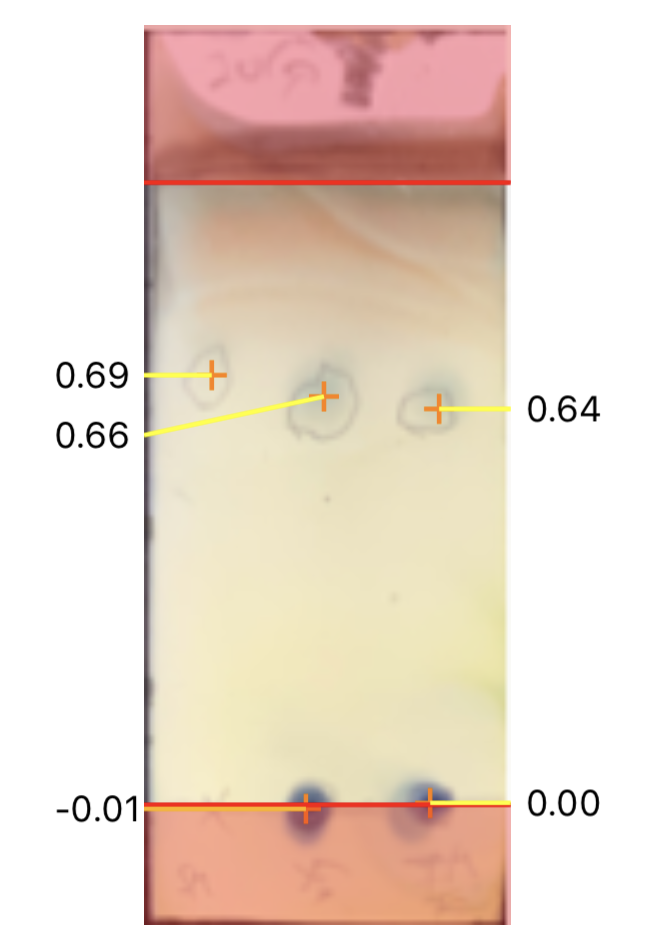
\includegraphics[clip, width=1.0cm]{imgs6/tlc-e20.PNG}
\hspace{1.6cm} 20分
\end{center}
\end{minipage}

\begin{minipage}{0.19\hsize}
\begin{center}
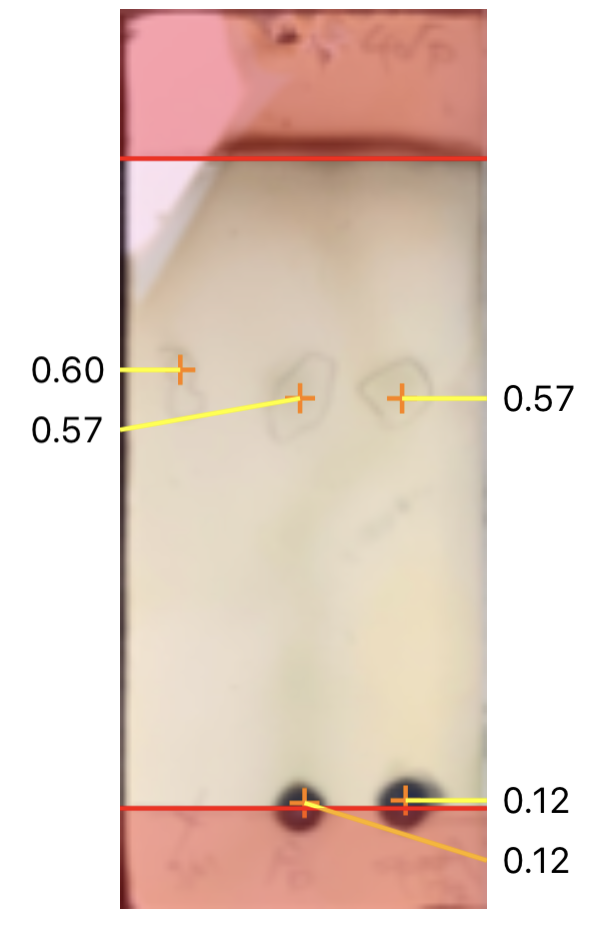
\includegraphics[clip, width=1.0cm]{imgs6/tlc-e40.PNG}
\hspace{1.6cm} 40分
\end{center}
\end{minipage}

\end{tabular}
\caption{リンモリブデン酸}
\end{center}
\end{figure}

\begin{figure}[htbp]
\begin{center}
\begin{tabular}{c}

\begin{minipage}{0.19\hsize}
\begin{center}
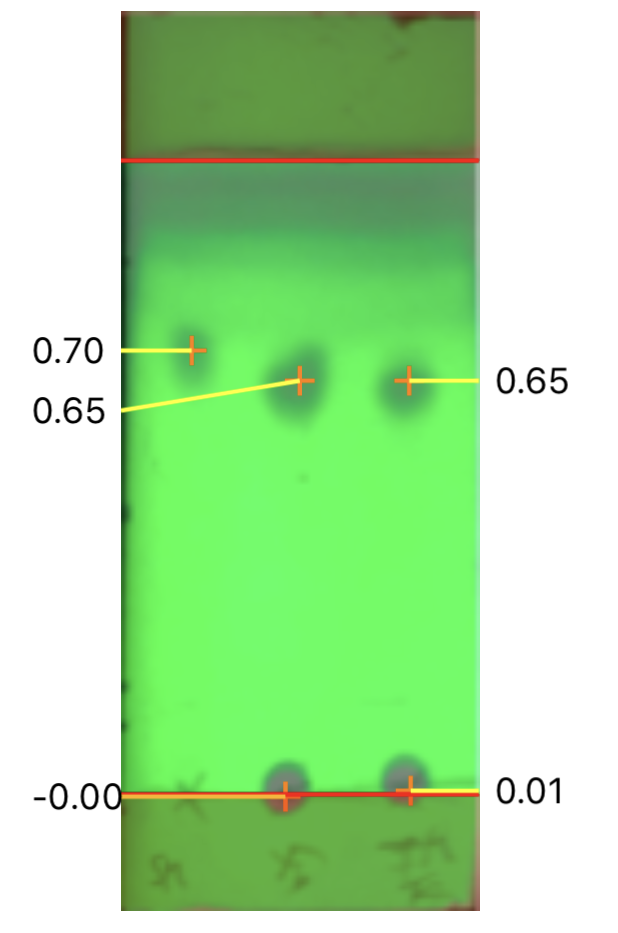
\includegraphics[clip, width=0.3\linewidth]{imgs6/tlc-u20.PNG}
\hspace{0.2cm} 20分
\end{center}
\end{minipage}

\begin{minipage}{0.19\hsize}
\begin{center}
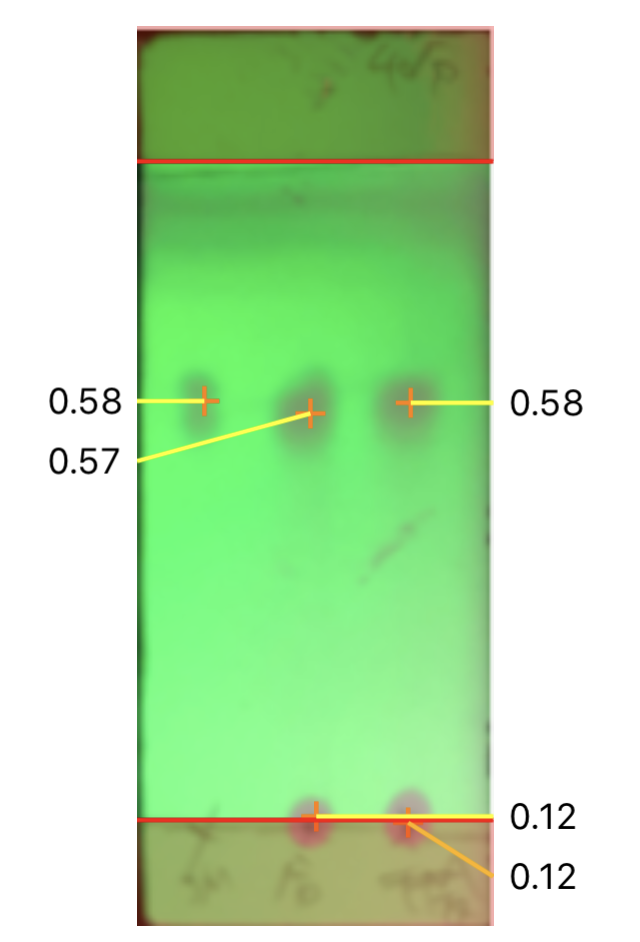
\includegraphics[clip, width=0.3\linewidth]{imgs6/tlc-u40.PNG}
\hspace{0.2cm} 40分
\end{center}
\end{minipage}

\end{tabular}
\caption{UV}
\end{center}
\end{figure}
\subsection*{考察}
\subsection*{課題}

1-a. トリクロロエチルエステル化の反応機構を記せ。
\pict{imgs-k/hk1.jpeg}{10}
\pict{imgs-k/hk2.jpeg}{10}
求核性および脱離能の高いピリジンが触媒として働いている。

1-b. トリクロロエチルエステルとして保護する理由を述べよ。他の考えられる代表的なカルボン酸の保護基を挙げつつ、それぞれのケースで考えられる問題点と照らしながら説明すること。
1-c. スルホキシド体の酸化において、$\beta -$スルホキシド基が選択的に得られる理由を述べよ。またアミノ基の保護基としてフタルイミドを用いた場合の結果を予想せよ。
1-d. 環拡大反応の反応機構を記せ。カルボキシ基を保護しないで行った場合、どのような問題点が考えられる。
\begin{enumerate}
\item NMR・IRのスペクトルピークを帰属せよ。
\item 細菌の細胞壁合成経路を概説し、$\beta -$ラクタム系抗生物質とバンコマイシンの作用機序について構造式を使いながらそれぞれ簡単に説明せよ。
\item $\beta -$ラクタム系抗生物質とバンコマイシンに対する細菌の耐性獲得機構を、構造式を用いながらそれぞれ説明せよ。
\item 新規反応開発研究が医薬プロセス化学にどのようなインパクトを与えるか、またこれによって世界はどのように良くなっていくかについて、考察せよ。
\end{enumerate}


\begin{figure}[htpb]
  \centering
    \begin{tabular}{c}
 
%----- y = sin(x) -----
 
      \begin{minipage}{0.47\hsize}
        \centering
          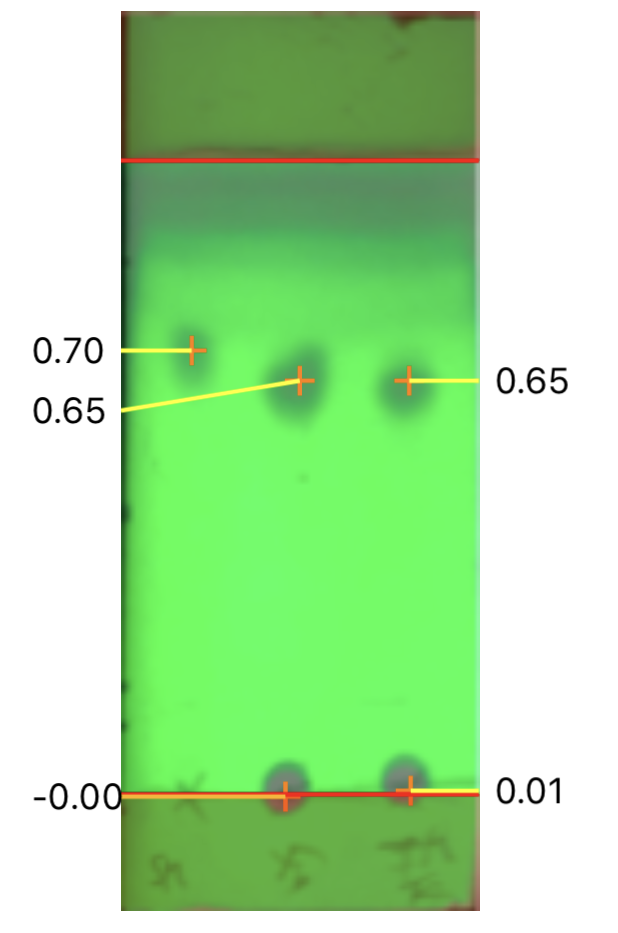
\includegraphics[keepaspectratio, scale=0.60, angle=0]
                          {imgs6/tlc-u20.png}
                          \caption{$y=\sin(x)$ のグラフ.}
                          \label{fig:sin_x}
      \end{minipage}
 
%--- 中央スペース
 
      \begin{minipage}{0.06\hsize}
        \hspace{2mm}
      \end{minipage}
 
%----- y = sin(2x) -----
 
      \begin{minipage}{0.47\hsize}
        \centering
          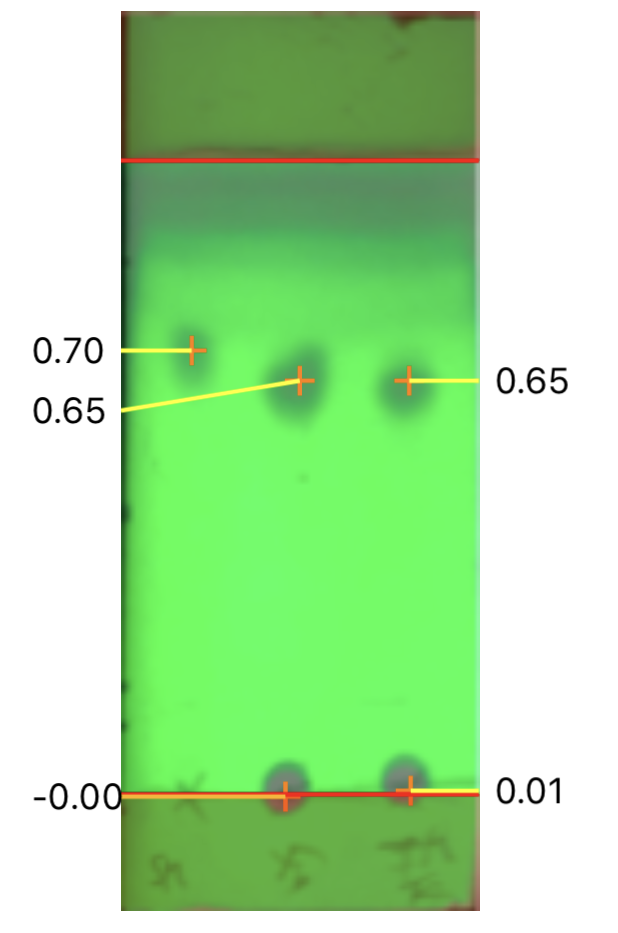
\includegraphics[keepaspectratio, scale=0.60, angle=0]
                          {imgs6/tlc-u20.png}
                          \caption{$y=\sin(2x)$ のグラフ.}
                          \label{fig:sin_2x}
      \end{minipage} \\
 
%--- 上下スペース
 
      \begin{minipage}{0.06\hsize}
        \vspace{10mm}
      \end{minipage} \\
 
 
%----- y = sin(3x) -----
 
      \begin{minipage}{0.47\hsize}
        \centering
          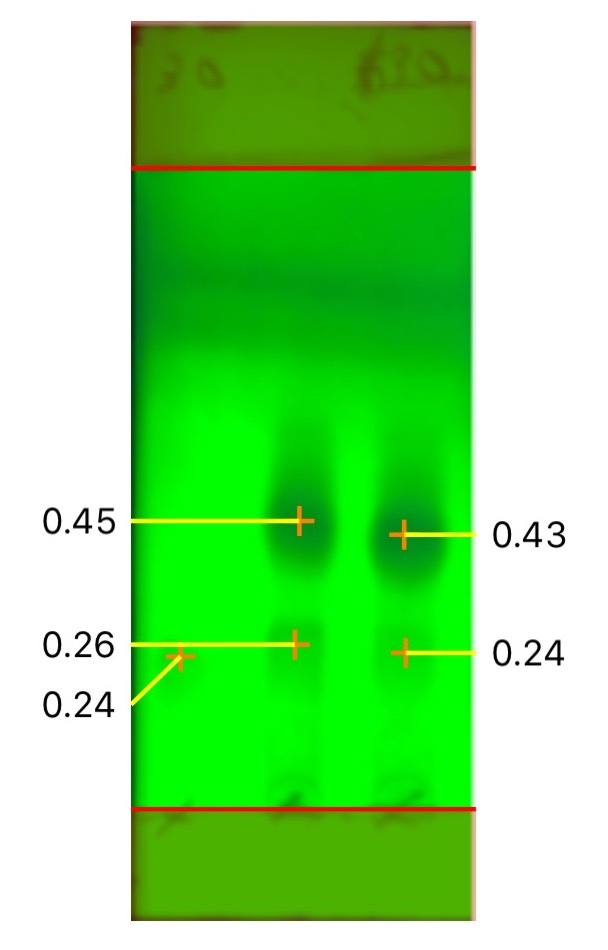
\includegraphics[keepaspectratio, scale=0.60, angle=0]
                          {imgs4/tlc1.JPG}
                          \caption{$y=\sin(3x)$ のグラフ.}
                          \label{fig:sin_3x}
      \end{minipage}
 
%--- 中央スペース
 
      \begin{minipage}{0.06\hsize}
        \hspace{2mm}
      \end{minipage}
 
 
%----- y = sin(4x) -----
 
      \begin{minipage}{0.47\hsize}
        \centering
          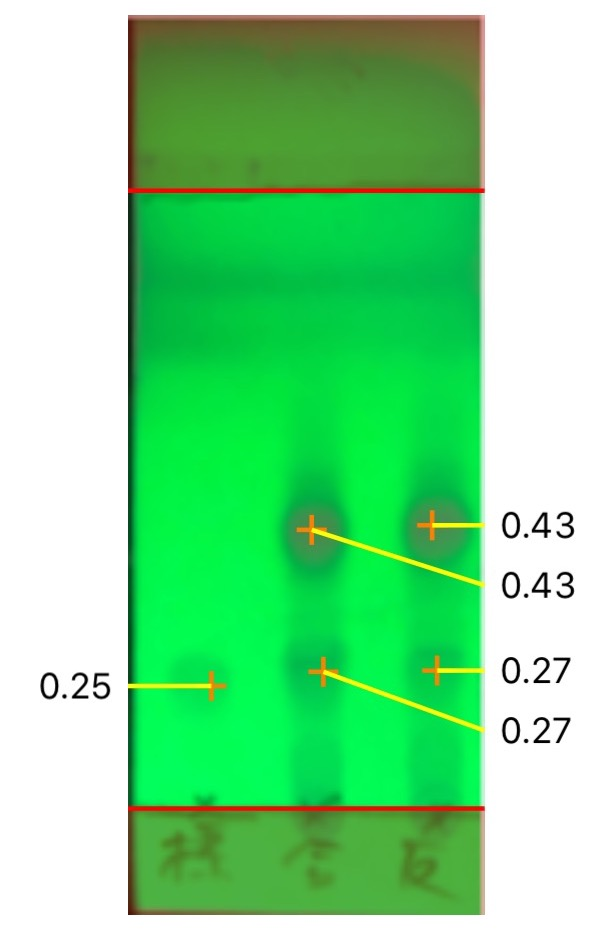
\includegraphics[keepaspectratio, scale=0.60, angle=0]
                          {imgs4/tlc4.jpg}
                          \caption{$y=\sin(4x)$ のグラフ.}
                          \label{fig:sin_4x}
      \end{minipage}
 
 
    \end{tabular}
\end{figure}  


\pict{imgs-k/btr.png}{10}

\end{document}